\section{CodeBsp}
\subsection{Circular Buffer}
Chap \ref{CircularBuffer} on Page \pageref{CircularBuffer}
\lstinputlisting[style=customC,linewidth=\linewidth]{code/CircularBuffer.c}
\clearpage

\subsection{Interrupt}
\subsubsection{Interrupt in C}
Chap \ref{InterruptC} on Page \pageref{InterruptC}
\lstinputlisting[style=customC,linewidth=\linewidth]{code/InterruptC.c}

\subsubsection{Multi-Interrupt in C }
Chap\ref{MultiInterruptC} on Page \pageref{MultiInterruptC}
\lstinputlisting[style=customC,linewidth=\linewidth]{code/MultiInterruptC.c}

\subsection{GPIO}
Chap \ref{GPIO} on Page \pageref{GPIO}\\
\begin{minipage}{0.5\linewidth}
    Example 8.1 (Push-button/LED Interface) Consider an 8-bitGPIO port, denoted
    as Port X (Px), with a momentary push-button SW1 connected to pin 0 (Px.0) and a
    light-emitting diode (LED) D1 connected to pin 1 (Px.1). A hardware setup for this
    example is illustrated in Fig. 8.5. Assume Px pins are by default GPIOs with direction
    and data registers at addresses PxDir and PxDat, respectively. Also assume that a
    direction bit set to “1” makes its corresponding port bit work as output, otherwise
    it will work as input. Provide a code fragment to properly configure the port and to
    toggle the LED whenever SW1 is depressed.
\end{minipage}
\begin{minipage}{0.5\linewidth}
    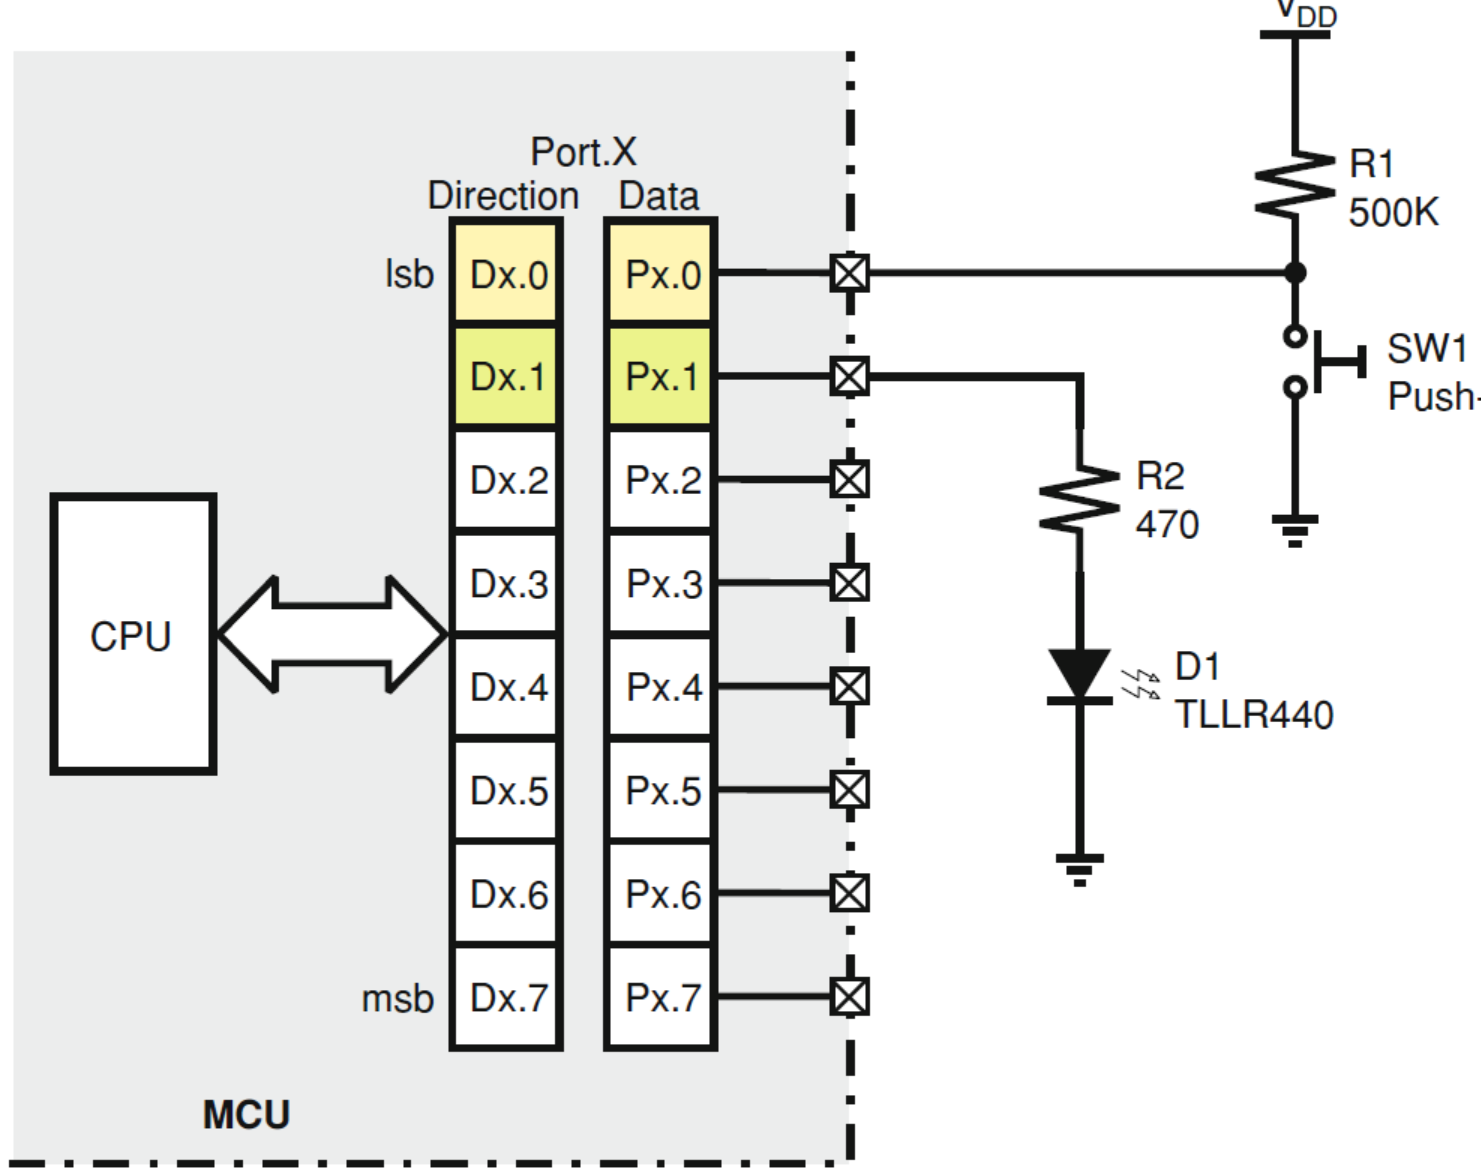
\includegraphics[width=\linewidth]{images/GPIOBsp}
\end{minipage}

\lstinputlisting[style=customasm,linewidth=\linewidth]{code/GPIO.c}

\begin{minipage}{0.5\linewidth}
    \subsection{Counting Debouncer }
    Chap\ref{CountingDebouncer} on Page \pageref{CountingDebouncer}
\end{minipage}
\begin{minipage}{0.5\linewidth}
    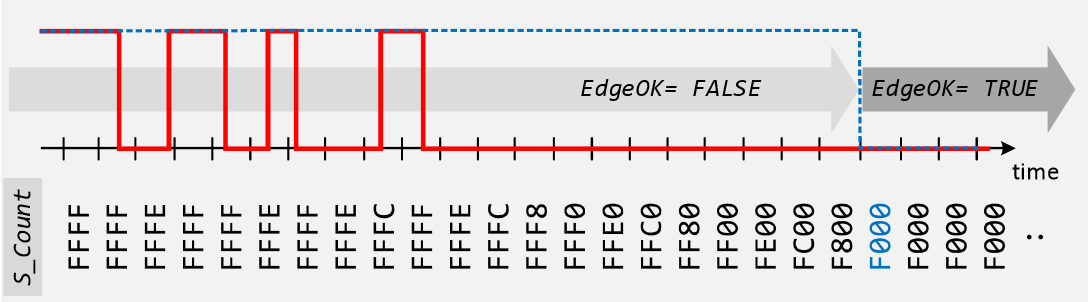
\includegraphics[width=0.9\linewidth]{images/CountingDebouncerTiming}
\end{minipage}
\lstinputlisting[style=customasm,linewidth=\linewidth]{code/CountingDebouncer.c}

\clearpage